% ==========================================================
% PneumoFusionNet - Term Project Report (Trimester 8)
% IIT Guwahati | B.Sc. Data Science & AI
% Ashutosh Yadav (Roll: 23035010693)
% ==========================================================

\documentclass{article}
\usepackage{spconf,amsmath,amssymb,graphicx,hyperref}
\usepackage{booktabs}
\usepackage{enumitem}
\usepackage{needspace}
\usepackage{tikz}
\usepackage{xcolor}
\usepackage{tcolorbox}
\usepackage{pgfplots}
\pgfplotsset{compat=1.18}
\usetikzlibrary{arrows.meta, positioning}

\hypersetup{colorlinks=true, linkcolor=blue!70!black,
            citecolor=blue!70!black, urlcolor=teal}
\tcbuselibrary{skins}
\definecolor{successgrn}{RGB}{39,174,96}

\def\x{{\mathbf x}}
\def\L{{\cal L}}

% ---------
\title{PneumoFusionNet: A Multimodal Deep Learning System
for Pneumonia Detection Using Chest X-Rays and Clinical Reports}

\name{Ashutosh Yadav (Roll Number: 23035010693)}

\address{
  Term Project Report (Trimester 8)\\[0.4em]
  B.Sc.\ (Honours) Data Science and Artificial Intelligence\\
  Indian Institute of Technology Guwahati, India\\
  \texttt{ashutosh@op.iitg.ac.in}
}

% ==========================================================
\begin{document}
\ninept
\maketitle

% ==========================================================
\begin{abstract}
This report presents \textbf{PneumoFusionNet}, a multimodal deep learning system
that detects pneumonia by combining chest X-ray images with clinical report text.
The system was built and tested on the restricted \textbf{MIMIC-CXR} hospital
dataset, which required completing a CITI research ethics course and signing a
Data Use Agreement (DUA) with PhysioNet to access.

We went through three stages: (1) a small 139-patient pilot using a ResNet50
image model with custom attention modules, (2) adding clinical text through a
\textbf{Bio\_ClinicalBERT} text encoder while carefully removing the doctor's
final diagnosis from the report to avoid cheating, and (3) scaling up to 854
chest X-ray images with three different preprocessing experiments.

Adding clinical text improved the AUC score by \textbf{+3.7\%} over the
image-only model. The best result on the scaled dataset was AUC \textbf{0.835}.
We found that ResNet50 (trained on everyday photos) does not transfer well to
medical X-rays, and our earlier high results on public datasets were partly
due to data leakage and very small, clean test sets.

\textbf{Index Terms-} Multimodal Deep Learning, Chest X-Ray, Bio\_ClinicalBERT,
Attention, Label Leakage, MIMIC-CXR.
\end{abstract}

\begin{keywords}
Pneumonia Detection, Multimodal Learning, MIMIC-CXR, ClinicalBERT, ResNet50
\end{keywords}

% ==========================================================
\section{Introduction}
% ==========================================================

Pneumonia is one of the top causes of death worldwide. Doctors use chest X-rays
to diagnose it because X-rays are fast and widely available. However, reading a
chest X-ray is not easy. The same cloudy patch in a lung can look like pneumonia,
fluid buildup, or a collapsed lung section. Even experienced radiologists
sometimes disagree. This is why building a reliable AI system for pneumonia
detection is both challenging and important.

Recent AI models have shown promise in reading chest X-rays
automatically~\cite{rajpurkar2017chexnet}. But image-only models ignore the
clinical context that every doctor uses-things like the patient's symptoms,
history, and test results. Adding radiology report text should help, but there
is a well-known trap: the last section of every radiology report (called
\texttt{IMPRESSION}) contains the doctor's final written diagnosis. If a model
reads this section during training, it is simply memorising the answer rather
than learning to diagnose. This is called \textbf{label leakage}, and it makes
the model useless in the real world.

\begin{tcolorbox}[colback=red!4!white, colframe=red!60!black,
                  title=What is Label Leakage?, fonttitle=\small\bfseries]
\small
A radiology report looks like this:\\[4pt]
\textbf{INDICATION:} Patient with fever and cough.
  \textcolor{successgrn}{\checkmark\ Used for training}\\
\textbf{FINDINGS:} Consolidation in left lower lobe.
  \textcolor{successgrn}{\checkmark\ Used for training}\\
\textbf{IMPRESSION:} Pneumonia confirmed.
  \textcolor{red}{\textbf{$\times$\ Removed before training}}\\[4pt]
If the model sees the IMPRESSION section, it just reads the answer.
We remove it completely so the model has to learn from actual evidence.
\end{tcolorbox}

This project builds PneumoFusionNet, a system that combines image and text
inputs while carefully removing the IMPRESSION section. It is adapted from a
2025 published paper~\cite{frontiers2025pneumofusion} and tested on the
MIMIC-CXR clinical database~\cite{johnson2019mimic}.

\textbf{Report outline:} Section~2 states the problem and goals. Section~3
explains the system design. Section~4 shows results. Section~5 discusses
what worked and what did not. Section~6 concludes.

% ==========================================================
\section{Problem Statement and Objectives}
% ==========================================================

\subsection{Problem Statement}

X-ray images alone are often not enough to reliably diagnose pneumonia,
especially when the signs are subtle. But simply adding the radiology report
text leads to label leakage (as explained above). The challenge is:
\textit{How do we use both the image and the report text together, without
the model cheating by reading the written diagnosis?}

A second challenge is the dataset itself. MIMIC-CXR is a restricted hospital
database. To use it, we had to:
\begin{itemize}[noitemsep, leftmargin=*]
  \item Complete the CITI Program training on human subjects research ethics.
  \item Sign a Data Use Agreement (DUA) with PhysioNet.
  \item Wait for credentialed access to be approved.
\end{itemize}
This process took several weeks but is required to ensure responsible use of
real patient data.

\subsection{Objectives}

\begin{enumerate}[noitemsep, leftmargin=*]
  \item Build an image-only classifier using ResNet50 with custom attention
        modules, tested on the 139-patient MIMIC-CXR pilot.
  \item Build an anti-leakage text pipeline that removes the IMPRESSION section
        and uses Bio\_ClinicalBERT to understand the remaining report text.
  \item Combine image features and text features into a single classifier.
  \item Scale up to 854 chest X-rays and test three different preprocessing
        approaches to find what works best on real clinical data.
  \item Understand the bottlenecks and plan the next steps.
\end{enumerate}

% ==========================================================
\section{System Design (Methodology)}
% ==========================================================

\subsection{Overall Pipeline}

The system works in two phases, as shown in Figure~\ref{fig:pipeline}.

\begin{figure}[h]
\centering
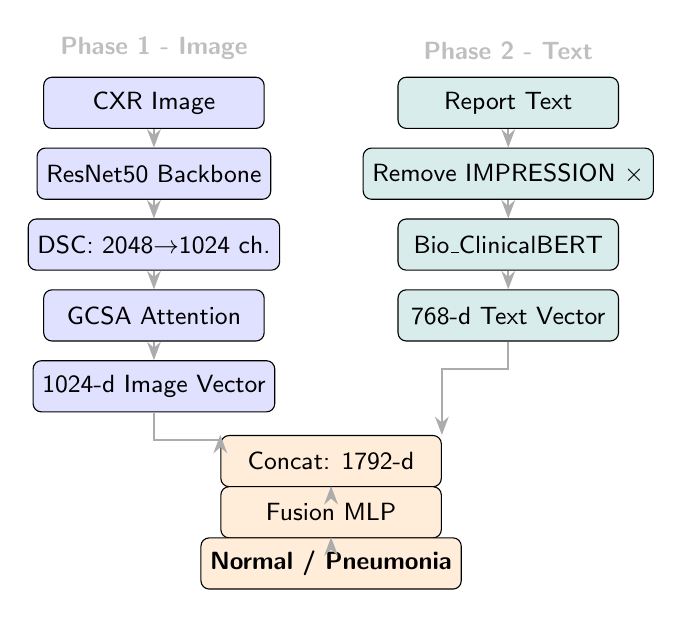
\begin{tikzpicture}[
  imgbox/.style={draw, rounded corners=3pt, fill=blue!12, align=center,
                 minimum height=0.65cm, minimum width=2.8cm,
                 font=\small\sffamily},
  txtbox/.style={draw, rounded corners=3pt, fill=teal!15, align=center,
                 minimum height=0.65cm, minimum width=2.8cm,
                 font=\small\sffamily},
  fusbox/.style={draw, rounded corners=3pt, fill=orange!15, align=center,
                 minimum height=0.65cm, minimum width=2.8cm,
                 font=\small\sffamily},
  arr/.style={-Stealth, thick, gray!65},
  lbl/.style={font=\small\bfseries\sffamily, text=gray!50}
]

%%-LEFT COLUMN: Image Branch --
\node[imgbox] (img)  at (0, 5.2) {CXR Image};
\node[imgbox] (res)  at (0, 4.3) {ResNet50 Backbone};
\node[imgbox] (dsc)  at (0, 3.4) {DSC: 2048$\to$1024 ch.};
\node[imgbox] (gcsa) at (0, 2.5) {GCSA Attention};
\node[imgbox] (iemb) at (0, 1.6) {1024-d Image Vector};

%%-RIGHT COLUMN: Text Branch --
\node[txtbox] (rep)   at (4.5, 5.2) {Report Text};
\node[txtbox] (strip) at (4.5, 4.3) {Remove IMPRESSION $\times$};
\node[txtbox] (bert)  at (4.5, 3.4) {Bio\_ClinicalBERT};
\node[txtbox] (temb)  at (4.5, 2.5) {768-d Text Vector};

%%-BOTTOM CENTRE: Fusion --
\node[fusbox] (cat) at (2.25, 0.65) {Concat: 1792-d};
\node[fusbox] (mlp) at (2.25, 0.0 ) {Fusion MLP};
\node[fusbox] (out) at (2.25,-0.65) {\textbf{Normal / Pneumonia}};

%% Column labels
\node[lbl, above=0.1cm of img]   {Phase 1 - Image};
\node[lbl, above=0.1cm of rep]   {Phase 2 - Text};

%% Arrows: image column (top-down)
\draw[arr] (img) -- (res);
\draw[arr] (res) -- (dsc);
\draw[arr] (dsc) -- (gcsa);
\draw[arr] (gcsa) -- (iemb);

%% Arrows: text column (top-down)
\draw[arr] (rep)  -- (strip);
\draw[arr] (strip) -- (bert);
\draw[arr] (bert) -- (temb);

%% Both branches merge into concat
\draw[arr] (iemb.south) -- ++(0,-0.35) -| (cat.north west);
\draw[arr] (temb.south) -- ++(0,-0.35) -| (cat.north east);

%% Fusion chain
\draw[arr] (cat) -- (mlp);
\draw[arr] (mlp) -- (out);

\end{tikzpicture}
\caption{PneumoFusionNet pipeline (vertical layout). Left column: the X-ray
image passes through ResNet50, DSC compression, and GCSA attention to give a
1024-d image vector. Right column: the report text has the IMPRESSION section
removed, then is processed by Bio\_ClinicalBERT to give a 768-d text vector.
Both vectors are joined (1792-d) and passed to a small MLP for final classification.}
\label{fig:pipeline}
\end{figure}

\textbf{Phase 1 - Image Classifier.}
The chest X-ray image is passed through the visual network. It is trained
from scratch on the MIMIC data until it converges. After training, it
saves the 1024-d feature vectors for every image.

\textbf{Phase 2 - Text Fusion.}
The image features are frozen (not updated). The cleaned report text is
processed by Bio\_ClinicalBERT. The image vector and text vector are
joined together and a small classifier is trained on top.

\subsection{Key Modules}

\subsubsection{ResNet50 Backbone}

ResNet50~\cite{he2016resnet} is a deep convolutional network pretrained on
ImageNet (a large collection of everyday photos). We adapted it to read
single-channel grayscale X-ray images by averaging its colour weights.
The early layers (which detect basic edges and textures) were kept frozen,
and only the deeper layers were fine-tuned on the medical data.

\subsubsection{Depthwise Separable Convolution (DSC)}

DSC is a compact convolution layer that compresses the ResNet50 output from
2048 channels down to 1024 channels using about half the number of
parameters of a standard convolution. This is important because medical
datasets are small, and fewer parameters means less risk of overfitting.
The mathematical operation is:
\begin{equation}
  \text{DSC}(\mathbf{X}) =
  \text{BatchNorm}\!\left(\text{ReLU}\!\left(
    \mathbf{W}_{1\times1} \ast (\mathbf{W}_{depth} \circledast \mathbf{X})
  \right)\right)
  \label{eq:dsc}
\end{equation}
where $\circledast$ is a channel-wise (depthwise) convolution and
$\ast$ is a $1\times1$ channel-mixing convolution.

\subsubsection{Global Context Spatial Attention (GCSA)}

GCSA is an attention mechanism that teaches the model \emph{where to look}
in the X-ray. It has two parts:

\textbf{Channel attention} decides \emph{which feature channels} are most
useful. It does this by squeezing the image into a single number per channel
(using average pooling and max pooling), then using a small neural network to
score each channel:
\begin{equation}
  \mathbf{A}_{channel} = \sigma\!\left(
    \text{MLP}(\text{AvgPool}(\mathbf{X})) +
    \text{MLP}(\text{MaxPool}(\mathbf{X}))
  \right)
  \label{eq:ach}
\end{equation}

\textbf{Spatial attention} decides \emph{which regions} of the image
to focus on. It collapses features across channels and runs a convolution:
\begin{equation}
  \mathbf{A}_{spatial} = \sigma\!\left(
    \text{Conv}_{7\times7}\bigl([\text{AvgCh}(\mathbf{X});\,\text{MaxCh}(\mathbf{X})]\bigr)
  \right)
  \label{eq:asp}
\end{equation}

The final attended feature map is:
\begin{equation}
  \hat{\mathbf{X}} = \mathbf{X} \times \mathbf{A}_{channel} \times \mathbf{A}_{spatial}
  \label{eq:gcsa}
\end{equation}

In simple terms: channel attention asks ``what features matter?'' and spatial
attention asks ``where in the image do they appear?''. Together they help the
model focus on the lung regions where pneumonia shows up.

\subsubsection{Bio\_ClinicalBERT Text Encoder}

Bio\_ClinicalBERT~\cite{alsentzer2019bert} is a BERT-based language model
that was pretrained on millions of clinical notes from the MIMIC-III hospital
database. It understands medical language far better than a general-purpose
model. We feed it the FINDINGS and INDICATION sections of the report
(after removing IMPRESSION) and use the 768-dimensional \texttt{[CLS]} token
output as a summary of the entire report. The last two layers of BERT are
fine-tuned during Phase 2 training.

\subsubsection{Fusion Classifier}

The 1024-d image vector and 768-d text vector are joined (concatenated)
to form a 1792-d combined vector. A small two-layer classifier predicts
the final label:
\begin{equation}
  \hat{y} = W_2 \cdot \text{ReLU}(W_1 \cdot [\mathbf{v}_{img} \| \mathbf{t}_{text}] + b_1) + b_2
  \label{eq:fusion}
\end{equation}

\subsection{Dataset and Setup}

\begin{tcolorbox}[colback=blue!4!white, colframe=blue!55!black,
                  title=Dataset Access - MIMIC-CXR-JPG (Restricted),
                  fonttitle=\small\bfseries]
\small
MIMIC-CXR is a real hospital chest X-ray database from Beth Israel Deaconess
Medical Center, USA. It is not publicly downloadable. To use it, we:
\begin{itemize}[noitemsep]
  \item Completed the CITI Program human subjects research training.
  \item Signed a PhysioNet Data Use Agreement (DUA).
  \item Applied for credentialed access (approved after verification).
\end{itemize}
All data was handled following the DUA terms - no patient-identifiable
information is stored or shared.
\end{tcolorbox}

\textbf{Pilot dataset (139 samples).}
We started with 139 patient studies from the MIMIC-CXR P10 folder.
This had 21 Pneumonia cases and 118 Normal cases - a very uneven split.
All view types (PA, AP, and Lateral X-rays) were included.
We used a 70\% train / 15\% validation / 15\% test split.

\textbf{Scale-up dataset (854 samples).}
For the scale-up, we expanded to 854 \emph{PA-view-only} frontal X-rays
(approximately 500 Pneumonia and 354 Normal).

\noindent\textit{Why PA-only?} During the pilot, we discovered a view bias:
the Pneumonia class had only 1 PA image but 12 AP and 5 Lateral images.
A model trained on mixed views can accidentally learn ``AP view = Pneumonia''
rather than actual lung disease. Filtering to PA-only removes this shortcut.

We also switched to \emph{patient-level splitting}: every image from the same
patient is kept in the same split (train, validation, or test). This prevents
the model from recognising a patient's anatomy rather than the disease.

\begin{table}[h]
\centering\small
\caption{Training settings for each experimental stage.}
\label{tab:hparams}
\begin{tabular}{lcc}
\toprule
\textbf{Setting} & \textbf{Pilot (139)} & \textbf{Scale-Up (854)}\\
\midrule
Backbone        & ResNet50         & ResNet50 \\
Image size      & $224\times224$   & $224\times224$ \\
Batch size      & 16               & 8 \\
Epochs          & 50               & 40 \\
Optimiser       & AdamW            & AdamW \\
Learning rate   & $10^{-4}$        & $10^{-4}$ \\
LR schedule     & Cosine           & Warmup + Cosine \\
Loss function   & Weighted BCE     & Cross-Entropy \\
Split method    & Stratified rows  & Patient-level groups \\
\bottomrule
\end{tabular}
\end{table}

% ==========================================================
\section{Experiments and Results}
% ==========================================================

\subsection{Setup}

\begin{itemize}[noitemsep, leftmargin=*]
  \item \textbf{Hardware:} NVIDIA RTX 3050 Laptop GPU (4\,GB), CUDA 11.2, Windows 11.
  \item \textbf{Software:} PyTorch 1.12.1, HuggingFace Transformers, Python 3.10.
  \item \textbf{Metrics:} AUC-ROC (main), Accuracy, F1 score, Sensitivity,
        Specificity.
\end{itemize}

\subsection{Pilot Results (139 Samples)}

We ran four experiments on the pilot data. Table~\ref{tab:pilot} shows
the results, and Figure~\ref{fig:auc_comparison} shows them visually.

\begin{table}[h]
\centering\small
\caption{Results on the 139-sample MIMIC-CXR pilot. All phases use the
same 70/15/15 split (seed~42).}
\label{tab:pilot}
\begin{tabular}{clccc}
\toprule
\textbf{Phase} & \textbf{What it uses} & \textbf{AUC} & \textbf{Accuracy} & \textbf{F1}\\
\midrule
1   & Image only (Imbalanced) & 0.667 & 76.2\% & 0.430 \\
1.1 & Image only (Balanced)  & \textbf{0.917} & \textbf{85.7\%} & \textbf{0.857} \\
2   & Image + Text (Imbalanced) & 0.704 & 81.0\% & 0.447 \\
2.1 & Image + Text (Balanced)  & \textbf{0.917} & 71.4\% & 0.708 \\
\midrule
\multicolumn{2}{l}{\textit{Gain from adding text (imbalanced)}}
  & $+$0.037 & $+$4.8\% & $+$0.017 \\
\bottomrule
\end{tabular}
\end{table}

\begin{figure}[h]
\centering
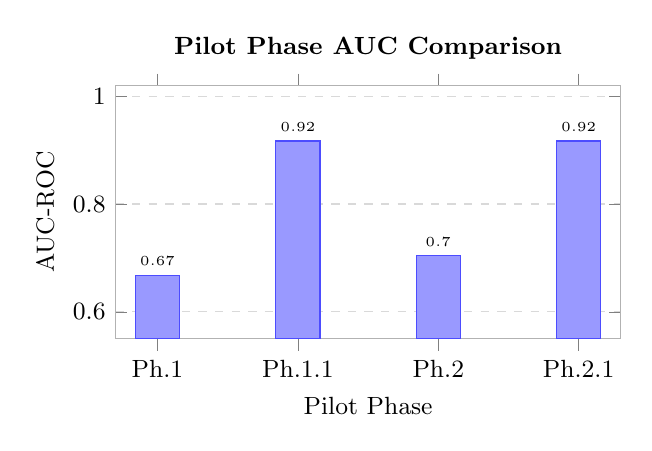
\begin{tikzpicture}
\begin{axis}[
  ybar, bar width=16pt,
  width=8cm, height=4.8cm,
  symbolic x coords={Ph.1, Ph.1.1, Ph.2, Ph.2.1},
  xtick=data,
  ymin=0.55, ymax=1.02,
  ylabel={AUC-ROC},
  xlabel={Pilot Phase},
  nodes near coords,
  nodes near coords align={vertical},
  every node near coord/.append style={font=\tiny},
  tick label style={font=\small},
  label style={font=\small},
  title={Pilot Phase AUC Comparison},
  title style={font=\small\bfseries},
  ymajorgrids=true, grid style={dashed, gray!30},
  axis line style={gray!60}
]
\addplot[fill=blue!40, draw=blue!70]
  coordinates {(Ph.1,0.667)(Ph.1.1,0.917)(Ph.2,0.704)(Ph.2.1,0.917)};
\end{axis}
\end{tikzpicture}
\caption{AUC across the four pilot phases. Balanced subsets (Ph.1.1, 2.1)
give high AUC but are based on only 7 test samples, making them unreliable.
On the imbalanced realistic set, adding text (Ph.2) gives a +0.037 AUC gain
over image-only (Ph.1).}
\label{fig:auc_comparison}
\end{figure}

\textbf{Important note on the balanced results.}
The balanced test set had only 7 samples. A single wrong prediction changes
accuracy by 14.3\%. A statistical test (Fisher's Exact, $p \approx 1.00$)
confirms that the difference between Phase~1.1 and Phase~2.1 is
\emph{not statistically meaningful}. The high AUC of 0.917 on balanced data
should be interpreted with caution - it was partly a result of the
very small and clean test set.

\subsection{Scale-Up Results (854 PA Images)}

We tested three different preprocessing approaches on the larger dataset.
Table~\ref{tab:scaleup} and Figure~\ref{fig:scaleup_bar} show the results.

\begin{table}[h]
\centering\small
\caption{Results on 854 PA-only MIMIC-CXR images across three preprocessing
versions.}
\label{tab:scaleup}
\begin{tabular}{lccccc}
\toprule
\textbf{Version} & \textbf{AUC} & \textbf{Acc.} & \textbf{Sens.} &
\textbf{Spec.} & \textbf{F1}\\
\midrule
\textbf{v1 Baseline}    & \textbf{0.835} & \textbf{69.4\%} & 65.3\% & 74.6\% & \textbf{0.69} \\
v2 Enhanced (failed)    & 0.725 & 58.5\% & 30.8\% & 85.2\% & 0.51 \\
v3 Fixed                & 0.714 & 64.2\% & 65.4\% & 63.0\% & 0.64 \\
\midrule
\textit{AP view test}   & 0.616 & 57.8\% & 84.8\% & 29.0\% & 0.53 \\
\bottomrule
\end{tabular}
\end{table}

\begin{figure}[h]
\centering
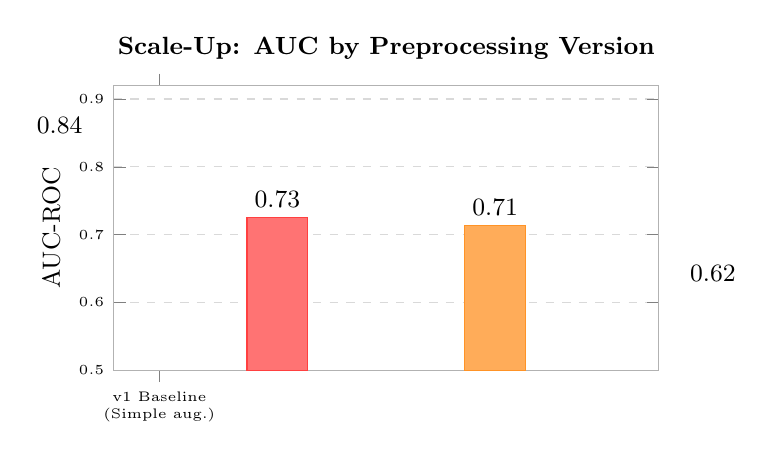
\begin{tikzpicture}
\begin{axis}[
  ybar, bar width=22pt,
  width=8.5cm, height=5.2cm,
  symbolic x coords={
    {v1 Baseline\\(Simple aug.)},
    {v2 Enhanced\\(ROI+CLAHE)},
    {v3 Fixed\\(Mixup+Smooth)},
    {AP view test}},
  xtick=data,
  xticklabel style={align=center, font=\tiny, text width=2cm},
  ymin=0.50, ymax=0.92,
  ylabel={AUC-ROC},
  nodes near coords,
  every node near coord/.append style={font=\small\bfseries},
  tick label style={font=\tiny},
  label style={font=\small},
  title={Scale-Up: AUC by Preprocessing Version},
  title style={font=\small\bfseries},
  ymajorgrids=true, grid style={dashed, gray!30},
  axis line style={gray!60}
]
%% Single addplot with per-bar colours via style lists is not trivial;
%% using separate plots without a legend is clean and unambiguous.
\addplot[fill=green!55!black!75, draw=green!70!black]
  coordinates {({v1 Baseline\\(Simple aug.)}, 0.835)};
\addplot[fill=red!55, draw=red!75]
  coordinates {({v2 Enhanced\\(ROI+CLAHE)},  0.725)};
\addplot[fill=orange!65, draw=orange!85]
  coordinates {({v3 Fixed\\(Mixup+Smooth)},  0.714)};
\addplot[fill=gray!40, draw=gray!60]
  coordinates {({AP view test},               0.616)};
%% No legend - bar labels on x-axis are self-explanatory
\end{axis}
\end{tikzpicture}
\caption{AUC scores for the three preprocessing versions tested on 854 PA-only
MIMIC-CXR images, plus an AP-view ablation. The simplest pipeline (v1) gave
the highest AUC. Adding lung-ROI cropping and CLAHE in v2 caused a 0.11 AUC
drop. Mixup and label smoothing in v3 did not recover fully.}
\label{fig:scaleup_bar}
\end{figure}

% ==========================================================
\section{Discussion}
% ==========================================================

\subsection{Did Adding Text Help?}

Yes. On the imbalanced pilot data (the realistic setting), adding clinical
report text improved AUC by \textbf{+3.7\%} and accuracy by \textbf{+4.8\%}.
This makes sense: the report text contains clues that the image alone cannot
show. For example, knowing that a patient has had a fever for three days and
is coughing helps the model treat an ambiguous lung shadow as more likely to
be pneumonia. All of these gains are genuine - the IMPRESSION section
was removed, so the model could not read the final diagnosis.

\subsection{Why Did v2 Preprocessing Fail?}

For v2, we tried two advanced preprocessing techniques:
\begin{itemize}[noitemsep, leftmargin=*]
  \item \textbf{Lung-region cropping} using the torchxrayvision library:
        The bounding box detection failed on 58\% of images (cut training
        data from 590 to 246 samples). Even successful crops often removed
        the lower-lobe areas where pneumonia is most common.
  \item \textbf{CLAHE contrast enhancement:} MIMIC-CXR has images from
        many different hospital scanners with different settings. CLAHE
        amplified the noise and differences between scanners, confusing the model.
\end{itemize}

The lesson is: techniques that work on clean benchmark datasets can easily
backfire on messy real hospital data. Keeping preprocessing simple (just
resize, flip, and mild augmentation) gave the best results.

\subsection{Why Were Earlier Results Misleadingly High?}

Our very first experiments on open-access public datasets showed 92\%
accuracy. This looked excellent. But those results were inflated by
two factors:
\begin{enumerate}[noitemsep, leftmargin=*]
  \item \textbf{Clean and balanced data:} Public datasets like the IU Chest
        X-Ray collection are pre-curated, balanced, and much easier than
        real hospital data. MIMIC-CXR reflects real clinical messiness.
  \item \textbf{Very small test sets:} On the 42-sample balanced pilot,
        the test set was only 7 images. A single wrong prediction changed
        accuracy by 14\%. These numbers are not statistically reliable.
\end{enumerate}
The true performance of the model on realistic, imbalanced hospital data
is much harder to achieve, as seen in the scale-up results.

\subsection{Limitations}

\begin{itemize}[noitemsep, leftmargin=*]
  \item \textbf{Not enough data:} 854 images is still too small. We need
        at least 2{,}000 PA images to get results we can trust for clinical use.
  \item \textbf{Low sensitivity:} The model correctly identifies only 65\%
        of actual pneumonia cases in the scale-up. A clinical screening
        tool needs at least 80\%.
  \item \textbf{Text fusion not yet scaled:} We only tested image+text
        fusion on the 139-patient pilot. The larger 854-image dataset
        has not yet had text fusion applied.
  \item \textbf{ResNet50 is not ideal for X-rays:} ResNet50 was originally
        trained on everyday photos (cats, dogs, vehicles). Chest X-rays are
        grayscale with very subtle intensity differences. The model struggles
        to pick up these fine details.
\end{itemize}

% ==========================================================
\section{Conclusion and Future Work}
% ==========================================================

In this project, we built PneumoFusionNet - a system that combines chest
X-ray images with clinical report text to detect pneumonia. We worked on real
restricted hospital data (MIMIC-CXR), which required completing CITI ethics
training and signing a PhysioNet Data Use Agreement (DUA) to access.

\textbf{What we achieved:}
\begin{itemize}[noitemsep, leftmargin=*, topsep=2pt]
  \item Built a two-phase image\,+\,text pipeline on restricted clinical data.
  \item Adding report text (IMPRESSION removed) gave \textbf{+3.7\% AUC}
        over image-only on the realistic imbalanced pilot.
  \item Found and fixed a view-bias (PA vs.\ AP) that was creating shortcuts.
  \item Simpler preprocessing (v1) consistently beat complex pipelines (v2/v3).
\end{itemize}

\textbf{Honest reflection:}
The high results on public datasets (92\% accuracy, AUC 0.917 on balanced
pilots) were due to: (1) clean/curated benchmark data, and (2) test sets as
small as 7 samples where one wrong prediction swings accuracy by 14\%.
On real MIMIC data with patient-level splits, results are lower but trustworthy.

\textbf{Core bottleneck - ResNet50 on X-rays:}
After trying attention modules, text fusion, balanced sampling, and three
preprocessing versions, the best scale-up AUC is still 0.835.
\textbf{ResNet50 was pretrained on everyday photos}, not medical images.
It struggles with grayscale X-rays that have very subtle intensity differences.

\needspace{5\baselineskip}
\textbf{Next steps:}
\begin{enumerate}[noitemsep, leftmargin=*, topsep=2pt]
  \item \textbf{Switch to DenseNet~\cite{huang2017densenet} with X-ray weights.}
        Use \textbf{torchxrayvision} pretraining (CheXpert, NIH, MIMIC-CXR)
        for domain-specific visual features.
  \item \textbf{Scale to 2{,}000+ PA images} (confidence margin $<\!\pm3\%$).
  \item \textbf{Run Phase~2 text fusion} on the larger dataset.
  \item \textbf{Add MIMIC-IV lab values} (WBC, CRP, Procalcitonin) as
        a third modality.
  \item \textbf{Grad-CAM on GCSA} so radiologists can inspect model focus.
\end{enumerate}

\subsection*{Artifacts and Code}
\begin{itemize}[noitemsep, leftmargin=*, topsep=2pt]
  \item \textbf{Code:}
    \href{https://github.com/Ashutosh-yadav0001/PneumoFusionNet}%
    {\texttt{github.com/Ashutosh-yadav0001/PneumoFusionNet}}
  \item \textbf{Pilot Notebooks (4):} \texttt{mimic/mimic\_pilot\_139/Notebooks/}
  \item \textbf{Scale-Up Notebooks (v1--v3):}
    \texttt{mimic/1000\_dataset/notebooks\_scaleUp/}
  \item \textbf{Results:} ROC curves, confusion matrices, training histories
    under \texttt{mimic/outputs/} and \texttt{mimic/1000\_dataset/outputs/}
  \item \textbf{Data Scripts:} \texttt{expand\_dataset\_pa.py},
    \texttt{generate\_paired\_metadata.py}, \texttt{train\_balanced\_scaleUp.py}
  \item \textbf{Video Demo:} [Link to be added after upload]
\end{itemize}

% ==========================================================
% References on their own clean page
% ==========================================================
\clearpage          % flush all floats before starting new page
\small              % slightly smaller font for references

\begin{thebibliography}{9}

\bibitem{rajpurkar2017chexnet}
P.~Rajpurkar et al., ``CheXNet: Radiologist-Level Pneumonia Detection on
Chest X-Rays with Deep Learning,'' \emph{arXiv:1711.05225}, 2017.

\bibitem{frontiers2025pneumofusion}
S.~Yu et al.,
``A multi-modal deep learning solution for precise pneumonia diagnosis:
the PneumoFusion-Net model,''
\emph{Frontiers in Physiology},
Sec.~Computational Physiology and Medicine,
vol.~16, Art.~1512835, 12~Mar.~2025.
\newblock DOI: \href{https://doi.org/10.3389/fphys.2025.1512835}{10.3389/fphys.2025.1512835}

\bibitem{alsentzer2019bert}
E.~Alsentzer et al., ``Publicly Available Clinical BERT Embeddings,''
\emph{arXiv:1904.03323}, 2019.

\bibitem{johnson2019mimic}
A.~E.~W.~Johnson et al., ``MIMIC-CXR, a de-identified publicly available
database of chest radiographs with free-text reports,''
\emph{Scientific Data}, vol.~6, no.~317, 2019.

\bibitem{he2016resnet}
K.~He, X.~Zhang, S.~Ren, and J.~Sun,
``Deep Residual Learning for Image Recognition,''
\emph{Proc.\ IEEE CVPR}, 2016, pp.~770--778.
\newblock \href{https://arxiv.org/abs/1512.03385}{arXiv:1512.03385}

\bibitem{huang2017densenet}
G.~Huang, Z.~Liu, L.~van~der~Maaten, and K.~Q.~Weinberger,
``Densely Connected Convolutional Networks,''
\emph{Proc.\ IEEE CVPR}, 2017, pp.~4700--4708.
\newblock \href{https://arxiv.org/abs/1608.06993}{arXiv:1608.06993}

\bibitem{irvin2019chexpert}
J.~Irvin et al., ``CheXpert: A Large Chest Radiograph Dataset with
Uncertainty Labels,'' \emph{Proc.\ AAAI}, 2019, pp.~590--597.

\end{thebibliography}

\end{document}
